\documentclass[pdftex,12pt,a4paper]{article}

\usepackage{graphicx}  
\usepackage[margin=2.5cm]{geometry}
\usepackage{breakcites}
\usepackage{indentfirst}
\usepackage{pgfgantt}
\usepackage{pdflscape}
\usepackage{float}
\usepackage{epsfig}
\usepackage{epstopdf}
\usepackage[cmex10]{amsmath}
\usepackage{stfloats}
\usepackage{multirow}

\renewcommand{\refname}{REFERENCES}
\linespread{1.3}

% REQUIRED FOR INSETYING SOME SHITASS ASSEMBLY CODE INTO TO LATEX BIATCH fuck this retarded thing, science my ass
\usepackage{listings}
\usepackage{xcolor}
\definecolor{codegreen}{rgb}{0,0.6,0}
\definecolor{codegray}{rgb}{0.5,0.5,0.5}
\definecolor{codepurple}{rgb}{0.58,0,0.82}
\definecolor{backcolthe}{rgb}{0.95,0.95,0.92}
\definecolor{CommentGreen}{rgb}{0,.6,0}
% bu salak seyin son satiri bosluk olunca calismiyor kendimi sikcem simdi
% Icine comment de konmuyor

\lstset{
    numbers=left,
    basicstyle=\small\ttfamily,
    numberstyle=\tiny,
    keywordstyle=\color{blue}\bfseries,
    keywordsprefix=B,
    language={[x86masm]Assembler},
    breaklines=true,
    commentstyle=\color{codegreen},
    keywordstyle=\color{blue},
    keywordstyle=[2]\color{orange},
    keywordstyle=[3]\color{codegray},
    numberstyle=\tiny\color{codegray},
    stringstyle=\color{codepurple},
    showtabs=false,
    frame=single,
    keepspaces,
}



\usepackage{mathtools}
%\newcommand{\HRule}{\rule{\linewidth}{0.5mm}}
\thispagestyle{empty}
\begin{document}
\begin{titlepage}
\begin{center}
\textbf{}\\
\textbf{\Large{ISTANBUL TECHNICAL UNIVERSITY}}\\
\vspace{0.5cm}
\textbf{\Large{COMPUTER ENGINEERING DEPARTMENT}}\\
\vspace{2cm}
\textbf{\Large{BLG 351E\\ MICROCOMPUTER LABORATORY\\ EXPERIMENT REPORT}}\\
\vspace{2.8cm}
\begin{table}[ht]
\centering
\Large{
\begin{tabular}{lcl}
\textbf{EXPERIMENT NO}  & : & 6 \\
\textbf{EXPERIMENT DATE}  & : & 27.11.2019 \\
\textbf{LAB SESSION}  & : & WEDNESDAY - 13.30 \\
\textbf{GROUP NO}  & : & G10 \\
\end{tabular}}
\end{table}
\vspace{1cm}
\textbf{\Large{GROUP MEMBERS:}}\\
\begin{table}[ht]
\centering
\Large{
\begin{tabular}{rcl}
150170062  & : & Mehmet Fatih YILDIRIM \\
150180704  & : & Cihat AKK\.{I}RAZ \\
150180705  & : & Batuhan Faik DER\.{I}NBAY \\
150180707  & : & Fatih ALTINPINAR \\
\end{tabular}}
\end{table}
\vspace{2.8cm}
\textbf{\Large{FALL 2019-2020}}

\end{center}

\end{titlepage}

\newpage


\thispagestyle{empty}
\addtocontents{toc}{\contentsline {section}{\numberline {}FRONT COVER}{}}
\addtocontents{toc}{\contentsline {section}{\numberline {}CONTENTS}{}}
\setcounter{tocdepth}{4}
\tableofcontents
\clearpage

\setcounter{page}{1}


\section{INTRODUCTION}

In this experiment, using 7-segment display and MSP430 microcontroller desired tasks are implemented in the experiment booklet. An interrupt handler(ISR), an timer interrupt handler(TISR) are used to perform these tasks.
\section{MATERIALS AND METHODS}

This experiment is conducted via using MSP430G2553 microprocessor. This microprocessor is programmed using Code Composer Studio according to desired tasks on the experiment handout. During coding below sources are used:

\begin{itemize}
    \item MSP430 Education Board Manual \cite{ref2}
    \item MSP430 Architecture Chapter 4 \cite{ref3}
    \item MSP430 Instruction Set \cite{ref4}
    \item Supplementary Chapter 6 General Purpose \cite{ref5}
    \item MSP430 User Guide - Chapter 8 \cite{ref5}
\end{itemize}

\subsection{Part 1}

In the first part of the experiment, the team was asked to write an infinite loop as the main program code in order to light up all four digits of the 7-segment display panel simultaneously, achieving an output as follows "0123" (See Figure \ref{fig:output-sevensegment}). 

\begin{figure}[H]
    \centering
    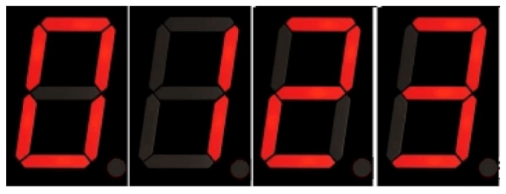
\includegraphics[width=0.5\textwidth]{0123_7segment.png}
    \caption{Sample Output of 4 Digit 7-Segment Display}
    \label{fig:output-sevensegment}
\end{figure}

To accomplish the assigned task, the code given in Figure \ref{code:part1_0123} was written. Let's go through the code and analyze the implementation:

\begin{itemize}
    \item Line 2-4: Initial setup of the ports 1 and 2 are done. All bits of port 1 and first 4 bits of port 2 are enabled. Then all the bits of port 1 are cleared. 
    \item Line 5-11: We set four registers each representing a digit of the display. From left to right R7, R6, R5 and R4 holds the values that is printed on the corresponding digits of the display. Even though the aim could have been achieved using only one register, because the next part involves modification of the values of each digit, this approach was chosen for flexibility. After moving the address of arr, that holds the binary values to output for each decimal number from zero to nine, to each register, their values were incremented respectively.
    \item Line 13-17: First the value stored in the memory address which is held by the corresponding register -in this case R4- is written to the port 1. Then the digit to display the value on port 1 is chosen using port 2. Notice here that hex value $0x08$ is $1000b$ and activates the rightmost digit of the display. It's also commented on the very first line in order to minimize unnecessary confusion. After selection of the outputs a no operation "NOP" instruction is executed in order to increase the delay between two digits. Without it, assuming the refresh rate of the digits are not able to catch up with the execution speed of the micro-controller, the display gets very low dark and unreadable. Then the output ports are cleared and got ready for the next digit to be displayed.
    \item Line 18-32: Same actions for the first digit are repeated for the remaining three digits in these lines. Note that the only differences are the aforementioned registers and its corresponding digit on port 2.
    \item Line 33: The program jumps back to the Main, completing a full cycle. Because it jumps back to the beginning without any exit condition, an infinite loop is achieved.
\end{itemize}

It is important to emphasize that because the data line for the display is shared among the digits, the illusion of a constant display is achieved by frequently flashing each digit of the display for a brief moment. None of the digits are light up exactly at the same time in order to achieve a constant display, else-wise, the number on the digits would have been the same.

\begin{figure}[H]
    \centering
    \begin{lstlisting}[language={[x86masm]Assembler}]
;r4 = 1, r5 = 10, r6 = 100, r7 = 1000, r15 = timer
Setup		        bis.b	#0FFh,  &P1DIR
			bis.b	#00Fh,  &P2DIR
			bic.b	#0FFh,  &P1OUT
			mov.w	#arr,   r4
			add     #3,     r4
			mov.w	#arr,   r5
			add     #2,     r5
			mov.w	#arr,   r6
			add     #1,     r6
			mov.w	#arr,   r7
			
Main		        mov.b	@r4,    &P1OUT
			mov.b	#08h,   &P2OUT
			nop
			clr     &P1OUT
			clr     &P2OUT
			mov.b	@r5,    &P1OUT
			mov.b	#04h,   &P2OUT
			nop
			clr     &P1OUT
			clr     &P2OUT
			mov.b	@r6,    &P1OUT
			mov.b	#02h,   &P2OUT
			nop
			clr     &P1OUT
			clr     &P2OUT
			mov.b	@r7,    &P1OUT
			mov.b	#01h,   &P2OUT
			nop
			clr     &P1OUT
			clr     &P2OUT
			jmp Main

arr .byte   00111111b, 00000110b, 01011011b, 01001111b, 01100110b, 01101101b, 01111101b, 00000111b, 01111111b, 01101111b
    \end{lstlisting}
    \label{code:part1_0123}
    \caption{Main Loop - Part 1}
\end{figure}

%%%%%%%%%%%%%%%%%%%%%%%
\newpage
\subsection{Part 2}

In this part, a chronometer which counts up continuously is implemented. When P2.5 is pushed or overflow occurs, the chronometer resets the time back to 0 and continues counting up.

In order to perform these operations, three code blocks are coded.

\begin{itemize}
    \item Timer Interrupt Subroutine
    \item Interrupt Subroutine
    \item BCD Convertion Subroutine
\end{itemize}

Let us go through the code and analyze the implementation.

% teşekkür ederiz var yok bey, kodları ve figürleri yerlerine göre ayırmışsınız.
\begin{itemize}
    \item Line 1-6: This is the setup sequence to enable interrupt functionality. Port 2's 7\textsuperscript{th} bit is set to 1, enabling interrupt when 7\textsuperscript{th} button is pressed. Remaining bits are set to 0 so I/O functions are selected for corresponding pins. Interrupt flag is set on a high-to-low transition for the 7\textsuperscript{th} bit. Then interrupt flags are cleared and interrupt is enabled for the micro-controller.
    
    \item Line 8-11: Initial setup of the ports 1 and 2 are done. All bits of port 1 and first 4 bits of port 2 are enabled. Then all the bits of port 1 are cleared.
    
    \item Line 13-18: \texttt{Set\_timer} function assigns the necessary values to TA0CTL, TA0CCR0 and TA0CCTL0 to have the timer exactly as needed. Let us examine them one by one.
    \newline
    TA0CTL is the configuration of the timer. It has 16 bits, the bits 15-10 of which is unused. Bits 9-8 should be 10 as using SMCLK is asked in lab booklet. Bits 7-6 should be 00 in order to set the input divider as /1 which will be okay in this case. Bits 5-4 should be 01 because "up mode" will be used.
    \newline
    TA0CCR0 consists of 16 bits and holds the value, up to which the timer will count. SMCLK's frequency is 1048576 Hz, meaning that at each second it operates that many times. The interrupts should be done once a centisecond, therefore the timer should count up to 1048576 divided by 100, which yields approximately 10486. Therefore, this value is assigned to TA0CCR0.
    \newline
    TA0CCTL0 consists of 16 bits as well and is the configuration of comp/cap mechanism. Bit 8 is set to 0 to choose compare mode. Bit 4 is set to 1 to enable interrupt request.
    
\end{itemize}
\begin{figure}[H]
    \centering
    \begin{lstlisting}[language={[x86masm]Assembler}]
setup_INT   bis.b       #040h,          &P2IE       
            and.b       #0BFh,          &P2SEL      
            and.b       #0BFh,          &P2SEL2
            bis.b       #040h,          &P2IES
            clr                         &P2IFG 
            eint    
;r4 = 1, r5 = 10, r6 = 100, r7 = 1000,
Setup	    bis.b       #0FFh,		&P1DIR
	    bis.b	#00Fh,		&P2DIR
	    bic.b	#0FFh,		&P1OUT
	    mov.b	#001h,		&P2OUT

Set_timer	; TA0CTL 15-10..100001x010
			; TA0CCR0	#10486d
			; TA0CCTL0  00??x?x00011x?x0
			mov.w	#01000010000b,	TA0CTL
			mov.w	#10486d,	TA0CCR0
			mov.w	#0000000000010000b,	TA0CCTL0

    \end{lstlisting}
    \label{code:part1delay}
    \caption{Setup sequences for Part 2}
\end{figure}

\begin{itemize}
    \item Line 28-53: Main function firstly calls BCD2Dec function to have the necessary values pointed by registers R4, R5, R6 and R7. Then, for each digit, the value stored in the memory address which is held by the corresponding register is written to the port 1. Then the digit to display the value on port 1 is chosen using port 2. Notice here that for instance, for the first digit, hex value $0x08$ is $1000b$ and it activates the rightmost digit of the display. After selection of the outputs, a no operation "NOP" instruction is executed in order to increase the delay between two digits. Without it, giving the refresh rate of the digits that are not able to catch up with the execution speed of the micro-controller, the display is dark and unreadable. Then the output ports are cleared and became ready for the next digit to be displayed. At line 53, the program jumps back to the Main, completing a full cycle. Because it jumps back to the beginning without any exit condition, an infinite loop is achieved.\end{itemize}
    
\begin{figure}[H]
    \centering
    \begin{lstlisting}[firstnumber=28][language={[x86masm]Assembler}]
Main		call	#BCD2Dec
			mov.b	@r4,		&P1OUT
			mov.b	#08h,		&P2OUT
			nop
			nop
			clr		&P1OUT
			clr		&P2OUT
			mov.b	@r5,		&P1OUT
			mov.b	#04h,		&P2OUT
			nop
			nop
			clr		&P1OUT
			clr		&P2OUT
			mov.b	@r6,		&P1OUT
			mov.b	#02h,		&P2OUT
			nop
			nop
			clr		&P1OUT
			clr		&P2OUT
			mov.b	@r7,		&P1OUT
			mov.b	#01h,		&P2OUT
			nop
			nop
			clr		&P1OUT
			clr		&P2OUT
			jmp		Main
    \end{lstlisting}
    \label{code:part1delay}
    \caption{Main Loop - Part 2}
\end{figure}

\begin{itemize}
    \item Line 55-60: The interrupt service routine (ISR) is called when Port 2 receives an interrupt signal. INT03 interrupt vector is instantiated and the interrupt handler routine in the memory location ISR is called. ISR disables the interrupts and zeros out the sec and csec values. Then clears the interrupt flag, re-enables the interrupts and returns from interrupt.
    
\end{itemize}
\begin{figure}[H]
    \centering
    \begin{lstlisting}[firstnumber=55][language={[x86masm]Assembler}]
ISR			dint
			mov.b 	#00h,  		sec
			mov.b	#00h,		csec
			clr		&P2IFG
			eint
			reti

    \end{lstlisting}
    \label{code:part1delay}
    \caption{Interrupt Subroutine - Part 2}
\end{figure}

\begin{itemize}
    \item Line 63-94: The timer interrupt service routine (TISR) is called when the timer sends an interrupt signal once a csec. INT09 interrupt vector is instantiated and the interrupt handler routine in the memory location TISR is called. TISR firstly disables the interrupts. Then, increments csec. After that, for each digit of csec value (in function names, they are referred to as csec, decisec(decsec), sec, decasec(deksec)), it does the following:
    \newline
    If the relevant digit is being incremented from the value 9, it jumps to the function which increments the digit right next to it (which is the rightmost digit that is greater in significance). Otherwise, it jumps to TISRend directly. TISRend re-enables the interrupts and returns from interrupt.
    \newline
    While doing all these operations, in order not to lose the value in R15, at top, its value is pushed to stack and at the very end, its value is popped back.
    \newline
    Note that even though generally the interrupt flag has to be cleared before returning from interrupt, it is not necessary in this case, because it is already automatically done.
    
\end{itemize}

\begin{figure}[H]
    \centering
    \begin{lstlisting}[firstnumber=63][language={[x86masm]Assembler}]
TISR		dint
			push	r15
			add.b	#1b,		csec
			mov.b	csec,		r15
			bic.b	#0F0h,		r15
			cmp		#0Ah,		r15
			jz		ADDDecSec
			jmp		TISRend

ADDDecSec	add.b	#010h,		csec
			bic.b	#00Fh,		csec
			mov.b	csec,		r15
			cmp		#0A0h,		r15
			jz		ADDSec
			jmp		TISRend

ADDSec		add.b	#001h,		sec
			bic.b	#0FFh,		csec
			mov.b	sec,		r15
			cmp		#0Ah,		r15
			jz		ADDDekSec
			jmp		TISRend

ADDDekSec	add.b	#010h,		sec
			bic.b	#00Fh,		sec
			mov.b	sec,		r15
			cmp		#0A0h,		r15
			jz		RESET

TISRend		pop 	r15
			eint
			reti

    \end{lstlisting}
    \label{code:part1delay}
    \caption{Timer Interrupt Subroutine - Part 2}
\end{figure}

\begin{itemize}
    \item Line 100-132: BCD2Dec function is called in Main to get the values of csec and sec which are set by TISR in BCD format, turn them into decimal format and set R4, R5, R6 and R7 so that they hold the addresses of values to be used when printing.
    \newline
    This is achieved by firstly, taking csec and sec (2 times each); secondly, if it is the second least significant bit of csec or sec that is being dealt with, performing right shift 4 times to get the second least significant bit of that variable (otherwise, least significant bit will already be had); thirdly, masking the value so that only the desired digit will be had and lastly, adding this value to be shown to the address of arr to have the address of the binary value in arr to be used to print the value to be shown and assigning it to the relevant register among R4, R5, R6 and R7.
    \newline
    While doing all these operations, in order not to lose the value in R14, at top, its value is pushed to stack and at the very end, its value is popped back.
\end{itemize}
%
\begin{figure}[H]
    \centering
    \begin{lstlisting}[firstnumber=100][language={[x86masm]Assembler}]
BCD2Dec		push 	r14

			mov.b	csec,	r14
			bic.b	#0F0h,	r14
			mov.w	#arr,	r4
			add.w	r14,	r4

			mov.b	csec,	r14
			rra.b	r14
			rra.b	r14
			rra.b	r14
			rra.b	r14
			bic.b	#0F0h,	r14
			mov.w	#arr,	r5
			add.w	r14,	r5


			mov.b	sec,	r14
			bic.b	#0F0h,	r14
			mov.w	#arr,	r6
			add.w	r14,	r6

			mov.b	sec,	r14
			rra.b	r14
			rra.b	r14
			rra.b	r14
			rra.b	r14
			bic.b	#0F0h,	r14
			mov.w	#arr,	r7
			add.w	r14,	r7

			pop		r14
			ret

    \end{lstlisting}
    \label{code:part1delay}
    \caption{BCD Conversion Subroutine - Part 2}
\end{figure}

\begin{itemize}
    \item Line 135-140: In these lines, necessary definitions are done. Firstly, an array of 10 elements is defined which holds the bit-wise values that turn on the corresponding LEDs of the 7-segment display in order to display decimal numbers. Then, 2 more variables sec and csec are initialized as 0 whose values will be displayed.
\end{itemize}
\begin{figure}[H]
    \centering
    \begin{lstlisting}[firstnumber=135][language={[x86masm]Assembler}]
;0, 1, 2, 3, 4, 5, 6, 7, 8, 9
arr			.byte	00111111b, 00000110b, 01011011b, 01001111b, 01100110b, 01101101b, 01111101b, 00000111b, 01111111b, 01101111b
arr_end
			.data
sec			.byte	00h
csec 		.byte 	00h
    \end{lstlisting}
    \label{code:part1delay}
    \caption{Definitions, variables - Part 2}
\end{figure}


\newpage
\section{RESULTS}%conc kısmı niye benim cümlelerim sen kimsin 
 
At the end of the first task, the team is succeeded in lit different digits of 7-segment display panel simultaneously. How this is implemented are mentioned detailed in the methods part. Although the brightness at first was slightly lower, brightness was increased by playing with the delay which enables every digit to stay visible just a little longer.

At the second part of the experiment, a chronometer is implemented. How this chronometer is implemented mentioned detailed in the methods part. At the end of the experiment, the team had a chronometer that has functionality counting up continuously. Also has a functionality that when pressed a declared reset button, sets timer to 0 and starts counting up again.

Team also gathered how the timer works in MSP430, how to set it up and use it.

\section{DISCUSSION}

In the first part, lighting up all of the digits at once is possible by showing all digits one after the other rapidly. Which is enough to trick human eye to think all of them are lit at the same time. This is how all of the screens work in today's world. Old televisions used to scan the image and display it on the screen as little parts going from top left to top right then second line and so on. 

Interrupts caused by the timer was the focus in the second part of the experiment. A timer outside of the processor creates much better solutions for delaying program executions, computing are done related to time and so on. Before a delay can be achieved by writing correct value into a register and counting down from it in the main program. This creates a lot of problems. Since the counting down is done by the processor your program cannot run simultaneously and you have to calculate the value that you are going to write to the register after changing your program. Since number of clock cycles that your program uses will change every time you add or remove an instruction. Another downside of simulating delay in the main program is that power inefficiency since processor will be running all the time rather than sleeping when unnecessary or running other useful calculations.



\newpage
%Please explain, analyze, and interpret what have you done during the  experiment. 
\section{CONCLUSION}
%It was not difficult at all. We just nailed it goddamnit.


As always, the team has successfully completed all tasks. A few problems are faced in during the lab session were: changing the timer flag during timer interrupt service routine and using byte instructions rather than word during moving or adding address values. Timer interrupt flag is risen by itself, interrupt is called then it goes down by itself again. We used to change it in the beginning of the session and timer used to stop counting after first iteration. Took us quite a while to figure this one out.

Another lesson that should be taken from the experiment is remembering that address values are always 16-bit words. Doing byte operations on them will result those values lose first 8-bit which results inaccurate calculations. 


\nocite{overleaf}
\nocite{reportGuide}
\newpage
\addcontentsline{toc}{section}{\numberline {}REFERENCES}

\bibliographystyle{unsrt}
\bibliography{reference}

\end{document}

